\documentclass[12pt,fleqn]{article}\usepackage{../../common}
\begin{document}
Uretici Hasimsal Aglar (Generative Adverserial Networks -GAN-)

Derin Ogrenme ustalarindan Yann Lecun GAN'leri ``son 10 senede yapay ogrenmede
gorulen en buyuk ilerleme'' olarak tarif ediyor. Burada haksiz degil. YSA'lar
ilk basta (geri gelisinden sonraki ilk evresinde de) bir resimde kedi, kopek ya
da ucak olup olmadigini siniflayabiliyordu. Yeni evrisimsel (convolutional) yapi
ile cetrefil goruntu iliskilerini ogrenip bunlari siniflama ozelligi kazandi,
fakat bunlar basit bir etikete bagli olarak denetimli (supervised) olarak
yapiyordu.

GAN'ler denetimsiz olarak egitilebiliyor, ve daha ilginci ``uretimsel
(generative)'' olarak kullanilabiliyor. Mesela pek cok goruntuye bakip yeni
goruntuler ureten bir GAN olabilir, ya da, sozel tarif verilince o tarifteki
soylenen goruntuyu ureten bir GAN olabilir! Oyle ya sonucta verilen girdi bir
takim reel sayilar iceren cok boyutlu vektorlerdir, bu sayilarin kelimeleri,
baska goruntuleri temsil etmesi mimari acisindan cok fark yaratmaz.

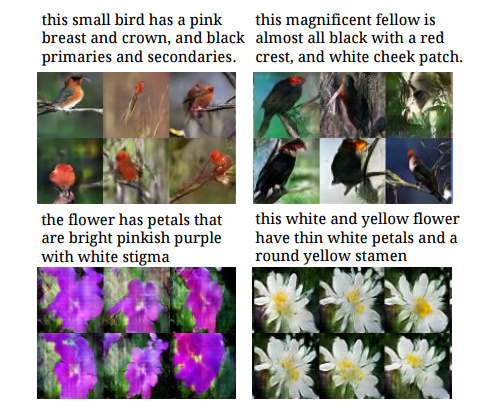
\includegraphics[width=20em]{gan_02.png}

Resimden resime tercume edebilmek, ``uretim yapmak'' elle cizilmis taslaklari
gercege cok yakin resimlere donusturmek, ya da tam tersi yonde gitmek mesela
bir uydunun cektigi sehir resmini haritasal yollar, evler semasina tercume
etmek, vs.

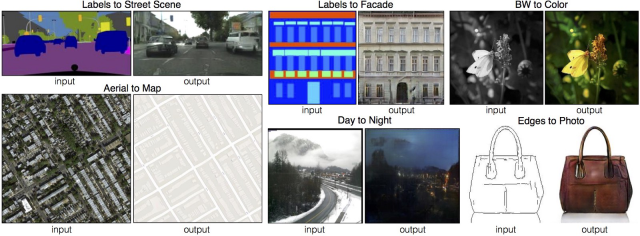
\includegraphics[width=20em]{gan_04.png}

Mimari

Simdi GAN'lerin nasil kurulduguna gelelim. Bir GAN yapisi kabaca bir kalpazan
(uretimsel) ve polis (ay�rta� -discriminator-) arasindaki iliskiyi
benzetilebilir. Ilk basta kalpazan polise bir sahte para gosterir, polis buna
sahte der. Bu noktada polis kalpazana onemli bir bilgi / geri besleme vermis
olur, kalpazan bu bilgiyi kullanarak bir sonraki sefere daha iyi sahte para
basmaya ugrasabilir. Bu dongu uzun sure devam ettirilir ta ki kalpazan isleri
iyice ilerletip polisi tamamen aldatabilinceye kadar. 

Imajlar baglaminda dusunelim simdi; sahte imajlar uretmek ve onlari
ayirdedebilmek. Ustteki anlatimdan bize iki tane ag gerektiginin
anlayabiliriz. Birincisi ayirtac, bu aga imaj verilir, o da cevap olarak 0/1
olarak sahte / degil, dogru / yanlis seklinde bir cevap hesaplar. 

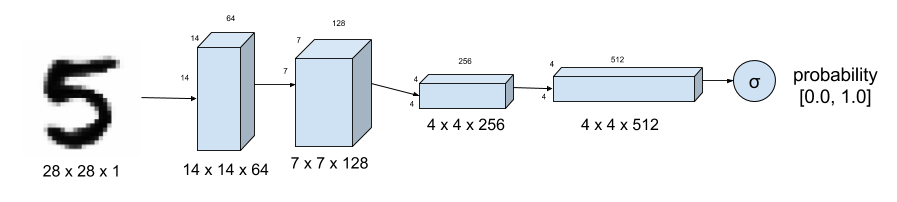
\includegraphics[width=20em]{gan_05.png}

Ikinci ag yapisi sahte imaj uretmeye ugrasiyor, ve bu uretimi cok iyi yapmaya
ugrasiyor. Peki girdi nedir? Gurultu! Ikinci aga 100 boyutlu gurultu verecegiz
(baska boyutlar da olabilir), ve bu gurultuyu isleyerek 28x28 boyutlarinda bir
imaj uretmesini bekleyecegiz. Bu dahiyane bir yontem. Agin hayal gormesini,
uretmesini istiyoruz, bu tur bir aga gurultu, ya da hiclikten daha iyi bir girdi
verilemezdi herhalde. Bu arada egitildikten sonra YSA'nin deterministik bir
yapida oldugunu unutmayalim, yani egitim bitince ayni gurultu iki kere verilince
ayni imaj uretilir. Degisik imajlar icin degisik gurultuler vermek lazim!
Degisik gurultu nasil olur? Gaussian bazli N(0,1) gurultu urettigimizi
dusunelim, bazen 0'in solundan bazen sagindan deger uretiyor olabiliriz. Muthis
olan YSA'nin egitim sirasinda bu tur gurultu farklarina hassas hale gelmesidir!

Ikinci ag

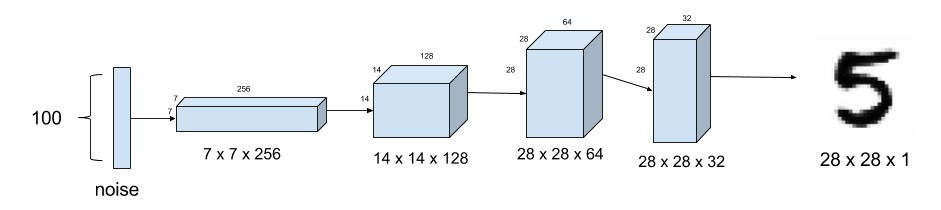
\includegraphics[width=20em]{gan_06.png}

Peki egitim verisi $X,y$ nedir, yani kaynak etiket nasil ayarlanir? Egitim
sirasinda gercek goruntuler arasindan belli sayida dosya toplanir, bunlar
``gercek'' yani 1 etiketi, ardindan elde en son olan uretece goruntu uretmesi
soylenir ve bu veriler 0 etiketi ile egitim verisine dahil edilir. Dikkat
edersek MNIST baglaminda mesela bu tabandan gelen 0,1,2,. gibi etiketleri
kullanmiyoruz, etiketleri kendimiz uretiyoruz. 

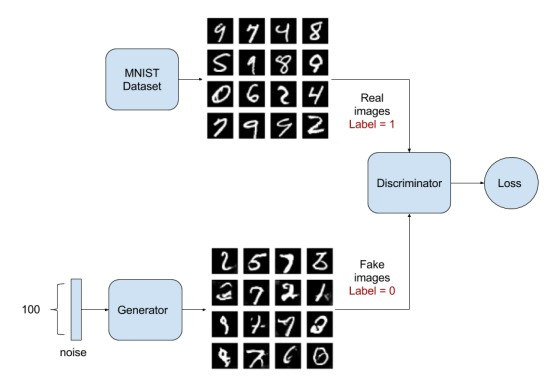
\includegraphics[width=20em]{gan_07.png}

Amac uretecin o kadar iyi hale gelmesi ki ayirtac gercek imaj ile hayali olani
birbirinden ayiredemesin. 

\inputminted[fontsize=\footnotesize]{python}{mnist_dcgan.py}

Egittikten sonra bir gurultu verip uretim yapalim,

\begin{minted}[fontsize=\footnotesize]{python}
import mnist_dcgan
generator, discriminator, gan = mnist_dcgan.get_model()
generator.load_weights("dcgan_generator_epoch_50.h5")
noise = np.random.randn(1,200)
pixels = generator.predict(noise).reshape((28,28))
plt.imshow(pixels)
plt.gray()
plt.savefig('gan_01.png')
\end{minted}

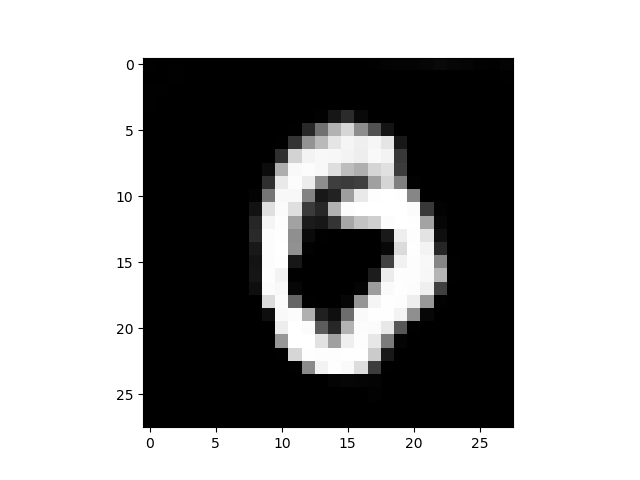
\includegraphics[width=20em]{gan_01.png}

Bir kez daha gurultu uretelim,

\begin{minted}[fontsize=\footnotesize]{python}
noise = np.random.randn(1,200)
pixels = generator.predict(noise).reshape((28,28))
plt.imshow(pixels)
plt.gray()
plt.savefig('gan_03.png')
\end{minted}

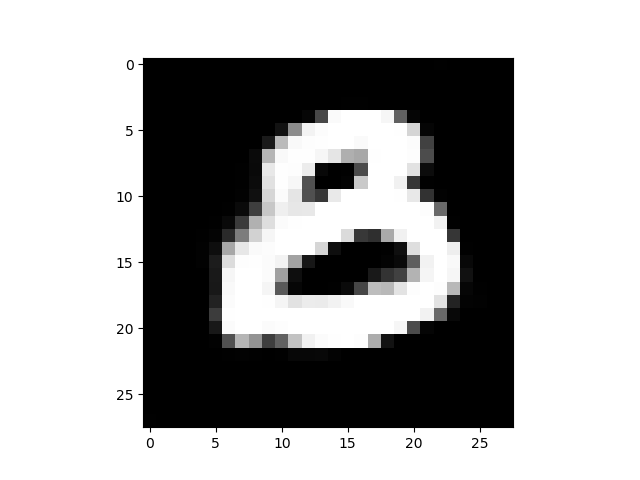
\includegraphics[width=20em]{gan_03.png}

Bu ciktilarin goruntusu ilginc degil mi? 



Kaynaklar

[1] \url{https://towardsdatascience.com/gans-n-roses-c6652d513260}

[2] \url{https://towardsdatascience.com/gan-by-example-using-keras-on-tensorflow-backend-1a6d515a60d0}


\end{document}
